\chapter{Характеристика объекта исследования}

Город Москва расширяет свои границы с каждым годом по причине увеличения населения. Новому населению требуется жилье. Развитие гражданского строительства достигло поселения Сосенское, где в настоящее время возводятся многоэтажные дома и проводятся инженерно-геологические исследования площадок для будущего построения жилых комплексов.
Поскольку территория изначально не была густо заселена, поэтому требуется более детальная изученность инженерно-геологических условий района. 
Исследования проводились проектно-изыскательной компанией ООО «ГеоГрадСтрой». Было определено геологическое строение района, изучены физические и физико-механические свойства грунтов основания. По предоставленным организацией данным была построена схематическая карта геологического строения.
В геологическом прошлом территория города Москвы и район исследования в том числе были покрыты ледниковыми покровами. Различают ледники двух эпох – московского и донского оледенения. Считается, что присутствие ледниковых покровов изменяет напряженно-деформированное состояние грунтов, они переуплотняются за счет веса вышележащего ледника, а после его отступления, грунты разгружаются. Эти процессы повлияли на настоящие физико-механические свойства грунтов и их напряженно-деформированное состояние.

Геологический разрез исследуемой территории был изучен на глубину 29,0 м, и представлен следующими стратиграфическими подразделениями:
1) Поверхность исследуемого участка покрыта почвенно-растительным слоем. Во всех скважинах встречены насыпные грунты (t H), представленные суглинком мягкопластичным, перекопанным, с прослоями песка, с включениями обломков бетона, битого кирпича, стекла, остатков древесины. Мощность насыпных грунтов составила 0,2-0,5 м.
2) Верхнечетвертичные покровные отложения (pr III) залегают повсеместно под насыпными грунтами и представлены глинами коричневыми с прослоями и пятнами серых глин, полутвердыми, местами до тугопластичных, с прослоями ожелезнений. Мощность глин составляет 1,6-1,7 м с абс. отм. подошвы 182,8-183,0 м.
3) Среднечетвертичные флювиогляциальные и озерно-ледниковые отложения московского горизонта (f,lg II ms) залегают ниже по разрезу, и представлены переслаивающейся толщей супесей, суглинков и песков. Пески мелкие, светло-коричневые, коричневые, средней плотности, глинистые, с прослоями суглинка и супеси, средней степени водонасыщения. Мощность песков составляет 0,2 м . Супеси светло-коричневые, коричневые, пластичные, слоистые, песчанистые пластичные, вскрыты в подошве флювиогляциальных отложений в виде прослоя мощностью 0,6 м. Суглинки коричневые, светло-коричневые, тугопластичные, пылеватые, слоистые, слагают основную толщу флювиогляциальных отложений в виде слоя мощностью 0,2-1,7 м. Общая мощность флювиогляциальных отложений московского горизонта составляет 1,3-1,7 м с абс. отм. подошвы 181,1-181,7 м.
4) Среднечетвертичные ледниковые отложения московского горизонта (g II ms) залегают под флювиогляциальными отложениями. Они представлены суглинками от коричневых до красновато-коричневых, тугопластичные, местами полутвердые, песчанистые, с прослоями супеси и песка, с включениями дресвы и щебня преимущественно карбонатных пород до 10-15%. В подошве с прослоями песка мелкого коричневого насыщенного водой. Их мощность колеблется от 0,9м до 2,1 м с абс. отм. подошвы 179,6-180,3 м.
5) Нижне-среднечетвертичные флювиогляциальные, ледниково-озерные, аллювиальные и озерные отложения донского-московского горизонта (f,lg I-II ds-ms) залегают повсеместно под флювиогляциальными и ледниковыми отложениями московского горизонта. Они представлены суглинками в кровле и в подошве, и глинами в средней части. Суглинки тугопластичные от светло-коричневых до зеленовато-коричнево-серых, тугопластичные, местами до полутвердых, песчанистые, слабо слоистые, с редкими включениями гравия и гальки, залегают преимущественно в кровле и подошве флювиогляциальных отложений. Мощность суглинков колеблется от 1,1 до 3,4 м. Глины серые, темно-серые, с зеленоватым оттенком, полутвердые, в кровле 0,2 м тугопластичные, слоистые, пылеватые, с единичными включениями гравия и гальки, преимущественно залегают в средней части толщи флювиогляциальных отложений донского-московского горизонта, и вскрыты всеми скважинами. Мощность глин составила 2,8-3,8 м. Общая мощность флювиогляциальных отложений донского-московского горизонта составляет 6,7-8,2 м с абсолютной отметкой подошвы 171,6-173,4 м.
6) Ниже залегают нижнечетвертичные ледниковые отложения донского горизонта (g I ds). Они представлены мощной толщей суглинков коричневых, до темно-серо-коричневых, полутвердых, в кровле 0,1-0,3 м тугопластичных, песчанистых, с включениями дресвы и щебня преимущественно карбонатных пород до 15%. Мощность этих суглинков составила 14,4 м, с абсолютной отметкой подошвы 157,2 м.
7) Завершают разрез на изученную глубину (29,0м) отложения нижнего отдела меловой системы (K1). Они представлены песками пылеватыми. Пески пылеватые, темно-серые, плотные, глинистые, слюдистые, насыщенные водой. Максимально вскрытая мощность этих песков составила 1,2 м.
Химический состав воды характеризуется как сульфатно-хлоридно-гидрокарбонатный магниево-кальциевый пресный с минерализацией 0,9 г/л, рН равен 7,9. Вода неагрессивная к бетону на портландцементе любых марок, слабоагрессивная к железобетонным конструкциям. Отмечается средняя коррозионная агрессивность к свинцовым и высокая к алюминиевым оболочкам кабелей.

Физико-механические свойства
Физико-механические свойства грунтов представлены в Таблице 1.


Также были проведены определения гранулометрического состава озерно-ледниковых и ледниковых отложений московского и донского горизонта ареометрическим методом. Определение проводилось по ГОСТ 12536-2014. В результате была построена треугольная диаграмма гранулометрического состава (рис.5).

\begin{figure}[h]
    {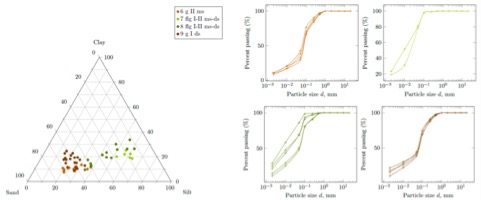
\includegraphics[scale=0.5]{ГранСостав.jpg}
    {рис 5. Результаты гранулометрического анализа: а) - треугольная диаграмма; б) - кумулятивные кривые.} 
     \caption\end{figure}
    
   
     Помимо определения основных физических и физико-механических свойств, был сделан рентгено-структурный анализ ледниковых и озерно-ледниковых отложений московского и донского горизонта в лаборатории кафедры инженерной и экологической геологии геологического факультета Московского университета им. М.В. Ломоносова. 

МИНЕРАЛОГИЧЕСКИЙ АНАЛИЗ ОБРАЗЦОВ

Студент: Фадеев Е.А.
Научный руководитель: Шанина В.В.
Дата поступления образцов: 27.11.2019
Дата составления отчета: 11.03.2020
Характеристика образцов: порошковая проба, количество – 4
Задачи исследования: количественный минеральный анализ 
Работы выполнены – инж. 1 кат. С.А. Гаранина, вед. инж. С.В. Закусин, 
ст.н.с., к.г.-м.н. В.В. Крупская

В качестве образцов использовались неориентированные препараты. Растертые предварительно образцы набивались в специальные кюветы без использования прессования при постоянном контроле качества поверхности для приготовления максимально разориентированного препарата.
Рентгенодифракционный анализ порошковых препаратов проводился при помощи рентгеновского дифрактометра ULTIMA-IV фирмы Rigaku (Япония). Рабочий режим – 40 кВ-40 mA, медное излучение, никелевый фильтр, диапазон измерений – 3-65о 2θ, шаг по углу сканирования 0.02о 2θ, фиксированная система фокусировочных щелей. Для ускорения съемки и повышения качества экспериментальных данных использовался полупроводниковый детектор нового поколения -  DTex/Ultra: скорость сканирования – 3о2θ/минуту 
Диагностика минерального состава проводилась методом сопоставления экспериментального и эталонных спектров из базы данных PDF-2 в программном пакете Jade 6.5, компании MDI. 
Количественный анализ. Количественный анализ осуществлялся методом полнопрофильной обработки рентгеновских картин от неориентированных препаратов по методу Ритвельда [2, 3] в программном продукте программе BGMN (www.bgmn.de). В основе метода лежит сопоставление расчетных и экспериментальных значений интенсивностей дифракционных отражений, которые измеряются в определенных точках дифрактограммы, полученной при пошаговом сканировании. В ходе анализа уточняются параметры элементарной ячеек всех ваз, содержащихся в смеси и определенных на предварительном этапе анализе, и координаты атомов каждой фазы. В результате сопоставления экспериментального и уточненного спектров рассчитывается весовое содержание фаз. Погрешность расчетов количественных содержаний по методу Ритвельда обычно принимается в 2-3%. Ошибка определения складывается из ошибок расчета для каждой фазы и дается в весовых процентах. При этом, для отдельных фаз ошибка определений будет отличаться и может составлять от 0.5 до 2-3%.
Результаты исследований.

Минеральный состав (вес. %):

	GJ6874	GJ6890	GJ6835	GJ6864
Смектит*	21.5	27.0	9.0	18.6
Хлорит	1.5	0.0	2.0	2.8
Иллит	10.2	6.0	8.3	4.9
Каолинит	4.6	4.6	1.4	3.5
Кварц	43.1	51.2	41.6	45.2
Плагиоклазы (Альбит)	8.1	4.6	17.0	3.8
КПШ (Микроклин)	10.2	5.7	10.3	5.6
Кальцит	0.0	0.0	4.4	6.4
Сидерит	0.4	0.0	0.3	0.0
Доломит	0.4	0.0	3.6	9.2
Анкерит	0.0	0.9	0.0	0.0
Роговая обманка	0.0	0.0	2.1	0.0

*Вероятно присутствие смешанослойного минерала – иллит-смектит с преобладанием смектитовых (набухающих) пакетов. Для точной диагностики требуется выделение глинистой фракции




Для определения характеристик переуплотнения грунта, были проведены испытания методом компрессионного сжатия. Компрессия – способность грунта сжиматься под постоянной, но ступенчато возрастающей нагрузкой без возможности его бокового расширения в условиях открытой системы. Компрессионное сжатие производилось по схеме, описанной в ГОСТ 12248-2010, в приборах ГТ1.1.4-01 ООО «НПП ГеоТек» (Пенза) при максимальных ступенях нагрузок до 2.5 МПа на образцах с естественной влажностью. 
Полученные данные были обработаны методами Казагранде и Беккера. По методу Казагранде строится полулагорифметический график зависимости коэффициента пористости от вертикального напряжения. Согласно методу Беккера, значение σp (напряжение предуплотнения) находится по графику зависимости увеличения работы на единицу объема (произведения давления на деформацию) от приращения вертикального давления.



Раньше все расчёты делались по СП. Только для уникальных сооружений использовали численное моделирование.

Сейчас даже для обычных домов часто используют моделирование. Эти параметры нужны чтобы более детально описывать поведение грунтов, вычислительные мощности позволяют.